\documentclass[
    journal=jctcce,
    layout=twocolumn
]{achemso}

\setkeys{acs}{
	abbreviations = false,
	articletitle  = false,
	keywords      = false,
	maxauthors    = 10,
	super         = true
}

% Comment below before submitting:
\let\titlefont\undefined
\usepackage[fontsize=11pt]{scrextend}
\usepackage[hidelinks,colorlinks,citecolor=blue]{hyperref}
%\flushbottom
% Up to this point

\usepackage{amsmath}
\usepackage{amssymb}
\usepackage[T1]{fontenc}
%
\usepackage[table]{xcolor}
\definecolor{lightgray}{gray}{0.85}
%
\usepackage{array}
\newcolumntype{L}{>{$}l<{$}}
\newcolumntype{C}{>{$}c<{$}}
\newcolumntype{R}{>{$}r<{$}}
%
\newcommand{\mt}[1]{\boldsymbol{\mathbf{#1}}}   % matrix symbol
\newcommand{\vt}[1]{\boldsymbol{\mathbf{#1}}}   % vector symbol
\newcommand{\tr}[1]{#1^\text{t}}                % transposition
\newcommand{\diff}[2]{\frac{\partial #2}{\partial #1}} % derivative
%\newcommand{\diff}[2]{\nabla_{#1}{#2}} % derivative
%\newcommand{\diff}[2]{\partial_{#1}{#2}} % derivative
\newcommand{\avg}[1]{\overline{#1}}             % average

%\listfiles

\author{Charlles R. A. Abreu}
\email{abreu@eq.ufrj.br}
\affiliation{Chemical Engineering Department, Escola de Quimica, Universidade Federal do Rio de Janeiro, Rio de Janeiro, RJ 21941-909, Brazil}

\title{Free Energy Computation and Property Reweighting From Multiple Time-Correlated Datasets}

\abbreviations{i.i.d., MC, MD, CLT, OBM, MSE, FEP, BAR, WHAM, MBAR, MICS}

\keywords{Free Energy Computation, Reweighting, Multistate, Uncertainty Estimation}

\begin{document}

%\begin{tocentry}
%Graphical Abstract
%\end{tocentry}

%\tableofcontents

\begin{abstract}
Abstract.
\end{abstract}

\section{Introduction}
\label{sec:introduction}

The propensity of a system to be at one state out of several possibilities can be quantified by comparing the free energy values. Besides, the rate at which a process occurs depends on the free energy profiles of realizable paths connecting the end states. For these reasons, free energy calculation is a task of paramount importance in Computational Chemistry \cite{Chipot_2007, Christ_2010, Hansen_2014} and plays a central role in applications such as protein-ligand binding \cite{Chodera_2011, Abel_2017, *Abel_2017_2, Cournia_2017, Mobley_2017}, protein folding \cite{Perez_2016}, adsorption and structural transitions in metal-organic frameworks \cite{Coudert_2008, Bousquet_2012, Ghysels_2013, Demuynck_2017}, and many others.

The present paper is concerned with the analysis of data produced by multiple simulations of a molecular system, aiming at estimating relative free energies and their uncertainties at all sampled states. A second goal consists in using these datasets to interpolate properties and uncertainties along a continuum of unsampled states. This tool is known as perturbation \cite{Zwanzig_1954} or reweighting \cite{McDonald_1967, *McDonald_1969}, depending on whether the interpolated quantity is a free energy or an ordinary ensemble average. The use of reweighting has, for instance, enhanced considerably our analysis of the thermodynamic behavior of some supercritical fluids \cite{Aimoli_2014, *Aimoli_2014_2, Nichele_2018}.

An important tool that fulfills all aforementioned goals is the Multistate Bennett Acceptance Ratio (MBAR) method \cite{Shirts_2008}. It can be viewed as an extension of the original BAR method \cite{Bennett_1976} or as a limiting case of the Weighted Histogram Analysis Method (WHAM) \cite{Ferrenberg_1989, *Kumar_1992}, with the benefits of dispensing with binning \cite{Tan_2012} and being born equipped with a proper uncertainty estimator \cite{Shirts_2008}. Indeed, the latter feature distinguishes MBAR from earlier binless versions of WHAM \cite{Bartels_2000, Souaille_2001}. The method descends from the work of \citeauthor{Kong_2003} \cite{Kong_2003} and other previous publications in the Statistics literature.\cite{Vardi_1985, Gill_1988, Geyer_1994, Lindsay_1995, Meng_1996}. Proper uncertainty estimators rely on the proof of specific Central Limit Theorems (CLT), which in the case of MBAR requires the samples to be devoid of autocorrelation. This often enforces the disposal of many blocks of correlated data before applying the method. Although most of the meaningful content of the sample remains after such \textit{subsampling} is done, the discarded data could be of use to reduce uncertainties and produce smoother profiles via reweighting.

Our aim here is to develop a method that shares the same goals as MBAR, but whose uncertainty estimator can cope with autocorrelation. Our new method relies on recent developments \cite{Flegal_2010, Buta_2010, Buta_2011, Doss_2014, Vats_2015, *Vats_2018, Tan_2015, Roy_2018} made on top of Geyer's Reverse Logistic Regression and Reweighting Mixtures  approach \cite{Geyer_1994}. We refer to the method as MICS, standing for Mixture of Independently Collected Samples.

We start our exposition with a contextualizing preamble, aiming at reviewing some basic concepts and establishing our train of thought. In this part, we offer an interpretation of MBAR as being equivalent to the analysis of an expanded-ensemble simulation \cite{Lyubartsev_1992} whose employed importance weights are unknown. This view complements a recent publication by \citeauthor{Shirts_2017} \cite{Shirts_2017} and hopefully contributes to the assimilation of both MBAR and MICS. After that, we present the new method itself, including its maximum-likelihood estimator for the free energies of the sampled states and its machinery for performing free-energy perturbation and reweighting. In all cases, proper uncertainty estimators are derived. In contrast to the usual index-based notation, we resort to differentiation in matrix notation (especially a matrix-based chain rule) and manage to derive remarkably compact expressions. Finally, we test MICS's performance in real-world applications, showing that it can lead to better estimates when compared to MBAR.

\section{Preamble}

\subsection{Importance Sampling, Uncertainty Analysis, and the Delta Method}
\label{sec:definitions}

Let $x$ represent the set of coordinates of a system which can be found at different equilibrium states. Each state $i$ is a statistical ensemble whose probability density is given by
\begin{equation}
\label{eq:state_prob_density}
\rho_i(x) = \frac{1}{Z_i} e^{-u_i(x)},
\end{equation}
where $u_i(x)$ is a reduced potential \cite{Shirts_2008, Chodera_2011_2} with known functional form, while $Z_i = \int e^{-u_i(x)}dx$ is the configurational integral of the system at state $i$. The ensemble average of a property $A(x)$ at state $i$ is defined as
\begin{equation}
\label{eq:ensemble average}
\langle A \rangle_i = \int A(x)\rho_i(x)dx.
\end{equation}

Assume that a sample of configurations $S_i = \{x_{i,k}\}_{k=1}^{n_i}$ has been obtained via importance sampling \cite{Allen_1987} (e.g. MC or MD) at state $i$. In this case, we can estimate $\langle A \rangle_i$ by a simple arithmetic average, that is,
\begin{equation}
\label{eq:average estimator}
\avg A_i = \frac{1}{n_i} \sum_{k=1}^{n_i} A(x_{i,k}).
\end{equation}

This estimator naturally extends to multivalued properties, such as vectors and matrices. It is valid whether the configurations in $S_i$ are independent and identically distributed (i.i.d.) or form a correlated time series. The difference resides in how to estimate the uncertainty of an average $\avg A_i$ or, more generally, of a function $h(\avg {\vt y}_i)$, where $\vt y(x)$ is a vector of configurational properties $\tr{[A(x) \; B(x) \; \cdots]}$. Let us define $\hat{\mt \Sigma}_{\avg{\vt y}_i}$ as the matrix of estimated asymptotic covariances amongst the entries of $\avg{\vt y}_i$. For an i.i.d. sample, the central limit theorem (CLT) states that such matrix can be obtained by simply dividing the sample covariances by the sample size, that is,
\begin{equation}
\label{eq:asymptotic covariance IID}
\hat{\mt \Sigma}^{\ast}_{\avg{\vt y}_i} = \frac{\sum\limits_{k=1}^{n_i} \left[\vt y(x_{i,k}) - \avg{\vt y}_i\right] \tr{\left[\vt y(x_{i,k}) - \avg{\vt y}_i\right]}}{n_i(n_i - 1)}.
\end{equation}

In the case of time-correlated samples, one can estimate asymptotic covariances via methods such as batching, spectral analysis, or regenerative simulations \cite{Geyer_1992, Alexopoulos_2006, Flegal_2010, Vats_2015, *Vats_2018}. Spectral methods usually provide better estimates than batching \cite{Flegal_2010}, but they are more computationally demanding, especially in the multivariate case \cite{Vats_2015, *Vats_2018}. In this context, the overlapping batch-mean (OBM) estimator \cite{Meketon_1984} is particularly appealing for being asymptotically equivalent to a spectral method while still being very efficient and easy to implement. For a sample $S_i$, it consists in defining $n_i-b_i+1$ overlapping blocks of size $b_i$. The average of $\vt y(x)$ is ${\avg{\vt y}}^b_{i,1} = \frac{1}{b_i} \sum_{k=1}^{b_i} \vt y(x_{i,k})$ for the first block and, for the remaining ones, they can be computed recursively by
\begin{equation*}
{\avg{\vt y}}^b_{i,j+1} = {\avg{\vt y}}^b_{i,j} + \frac{\vt y(x_{i,j+b_i}) - \vt y(x_{i,j})}{b_i}.
\end{equation*}

Then, the OBM estimator for $\hat{\mt \Sigma}_{\avg{\vt y}_i}$ becomes \cite{Meketon_1984}
\begin{equation}
\label{eq:obm asymptotic covariance}
\hat{\mt \Sigma}_{\avg{\vt y}_i} = \frac{b_i \sum\limits_{j=1}^{n_i - b_i + 1} ({\avg{\vt y}}^b_{i,j} - \avg{\vt y}_i) \tr{({\avg{\vt y}}^b_{i,j} - \avg{\vt y}_i)}}{(n_i - b_i)(n_i - b_i + 1)}.
\end{equation}

Asymptotic consistency requires that $b_i$ increases with $n_i$, and it is a common practice to make $b_i = \lfloor n_i^\nu \rfloor$ for some $0 < \nu < 1$, where $\lfloor \cdot \rfloor$ is the floor operator. As recommended by \citeauthor{Flegal_2010} \cite{Flegal_2010}, here we employ $\nu = 1/2$ and, therefore, $b_i = \lfloor \sqrt{n_i} \rfloor$.

Finally, once $\hat{\mt \Sigma}_{\avg{\vt y}_i}$ has been estimated, the mean square error (MSE) of $\avg A_i$ can be taken as the main-diagonal entry of $\hat{\mt \Sigma}_{\avg{\vt y}_i}$ corresponding to this property. In the case of $h(\avg{\vt y}_i)$, the MSE should be computed via the delta method \cite{Greene_2012}, from which
\begin{equation}
\label{eq:delta method}
\delta^2 h = \tr{\left(\diff{\avg{\vt y}_i} h\right)} \hat{\mt \Sigma}_{\avg{\vt y}_i}\left(\diff{\avg{\vt y}_i} h\right),
\end{equation}
where $\diff{\vt x}{}$ is the gradient operator with respect to a vector variable $\vt x$. The delta method is responsible for quantifying the propagation of uncertainties from $\avg{\vt y}_i$ to $h(\avg{\vt y}_i)$.

\subsection{Free Energy Computation and Property Reweighting}
\label{sec:fep and reweighting}

We are often interested in the difference between the reduced free energies of two states, defined as $\Delta f_{i,j} = f_j - f_i = - \ln (Z_j/Z_i)$. Due to the usual impossibility of computing absolute free energies, it is appropriate to define $f_i$ as a relative value with respect to a state~$0$, chosen as a common reference to all other states, so that $f_i = -\ln (Z_i/Z_0)$. We can thus rewrite Eq.~\eqref{eq:state_prob_density} as
\begin{equation}
\label{eq:state_prob_density_Z0}
\rho_i(x) = \frac{1}{Z_0} e^{-u_i(x)+ f_i}.
\end{equation}

The fact that $f_i$ can only be determined up to an additive constant will be assumed henceforth. By using a two-state method such as BAR \cite{Bennett_1976}, we can compute free-energy differences for the pairs of states whose sets of typical configurations \cite{Jarzynski_1997} overlap most considerably, and then piece them together to compute $\Delta f_{i,j}$ between poorly- or non-overlapping states. As another way of tackling overlap deficiency, we can define a reference state whose set of typical configurations encompasses those of all states of interest and then sample configurations state~$0$ itself, whose probability density is $\rho_0(x) = \frac{1}{Z_0} e^{-u_0(x)}$. After that, we are able to employ the perturbation formula
\begin{equation}
\label{eq:free energy perturbation}
f_u = -\ln \langle e^{u_0-u} \rangle_0,
\end{equation}
where $f_u$ is the relative free energy of a state whose reduced potential is $u(x)$. We are also able to perform reweighting by means of the identity \cite{Torrie_1977}
\begin{equation}
\label{eq:nbs sampling reweighting}
\langle A \rangle_u = \frac{\langle A e^{u_0 - u} \rangle_0}{\langle e^{u_0 - u} \rangle_0}.
\end{equation}

This strategy is known as \textit{non-Boltzmann sampling} \cite{Torrie_1977, Abreu_2006} due to the usually non-physical character of the sampled reference state, with the multicanonical approach \cite{Berg_1992} and the enveloping distribution method \cite{Christ_2007, *Christ_2008, *Christ_2009} being notable examples. Another technique of great relevance is the \textit{expanded ensemble} method \cite{Lyubartsev_1992}. It consists in combining a number $m$ of states whose distributions overlap and then doing importance sampling of a joint probability of configurations and states given by \cite{Nymeyer_2010}
\begin{equation}
\label{eq:expanded ensemble joint}
p_0(x, i) = \frac{1}{Z_0} e^{-u_i(x) + \eta_i},
\end{equation}
where $\vt \eta$ is a vector of arbitrary weighting factors. This procedure results in a sample $S = \{x_k,i_k\}_{k=1}^n$, where each configuration bears a state-indicating label. From Eq.~\eqref{eq:expanded ensemble joint}, one can derive the marginal probability of each state $i$ and the marginal density of configurations at state~$0$, respectively defined as $\pi_i = \int p_0(x,i)dx$ and $\rho_0(x) = \sum_{i=1}^m p_0(x,i)$. One can also obtain conditional probabilities via Bayes' theorem, $p_0(x,i) = p(x|i) \pi_i = p(i|x) \rho_0(x)$. Hence,
\begin{subequations}
	\label{eq:expanded ensemble probabilities}
	\begin{gather}
	\pi_i = \frac{Z_i}{Z_0} e^{\eta_i} = e^{\eta_i - f_i}, \label{eq:expanded ensemble prior} \\
	\rho_0(x) = \frac{1}{Z_0} \sum_{j=1}^m e^{-u_j(x) + \eta_j}, \label{eq:expanded ensemble evidence} \\
	p(i|x) = \frac{e^{-u_i(x) + \eta_i}}{\sum_{j=1}^m e^{-u_j(x) + \eta_j}}, \; \text{and} \label{eq:expanded ensemble posterior} \\
	p(x|i) = \frac{1}{Z_0} e^{-u_i(x) + f_i}. \label{eq:expanded ensemble likelihood}
	\end{gather}
\end{subequations}

The fact that $p(x|i) = \rho_i(x)$ proves that each individual state is sampled correctly. Once the sample $S$ has been generated, a simple estimator for the relative free energy of each state stems from Eq.~\eqref{eq:expanded ensemble prior} by making $\hat \pi_i = \frac{n_i}{n}$, where $n_i$ is the number of appearances of state $i$ in $S$. The result is
\begin{equation}
\label{eq:expanded ensemble histogram estimator}
\hat f_i = \eta_i - \ln \frac{n_i}{n}.
\end{equation}

However, we can derive a much better (Rao-Blackwellized \cite{Carlson_2016, Ding_2017}) estimator if we realize that $\pi_i = \int \rho_0(x) p(i|x) dx$, meaning that $\pi_i$ is the ensemble average of the marginal probability $p(i|x)$ at state $0$. The new estimator, which arises if we simply use Eq.~\eqref{eq:average estimator} to estimate such an average, is
\begin{equation}
\label{eq:expanded ensemble FEP estimator}
\hat f_i = -\ln \left[ \frac{1}{n}\sum_{k=1}^n \frac{e^{-u_i(x_k)}}{\sum_{j=1}^m e^{-u_j(x_k) + \eta_j}} \right].
\end{equation}

Note that the state-indicating labels in $S$ are neglected in both estimators. This is due to an essential feature of importance sampling: once sampled, every configuration contributes equally to an ensemble average. Finally, we can combine the results in Eq.~\eqref{eq:expanded ensemble probabilities} in order to show that an expanded ensemble distribution is actually a \textit{mixture model} \cite{Lindsay_1995, Marin_2005} composed of the distributions corresponding to the $m$ states, that is,
\begin{equation}
\label{eq:mixture ensemble}
\rho_0(x) = \sum_{i=1}^m \pi_i \rho_i(x).
\end{equation}

In this context, the vector $\vt \pi$ of state probabilities can be regarded as a composition. Moreover, since $\rho_0 = \frac{1}{Z_0}e^{-u_0}$, we can resort to Eq.~\eqref{eq:state_prob_density_Z0} for expressing the reduced potential of the mixture state as
\begin{equation}
\label{eq:mixture potential}
u_0(x) = -\ln \sum_{i=1}^m \pi_i e^{-u_i(x) + f_i}.
\end{equation}

With $\vt f$ replaced by its estimator $\hat{\vt f}$, this potential can be combined with Eqs.~\eqref{eq:free energy perturbation} and \eqref{eq:nbs sampling reweighting} so that perturbation and reweighting can be performed. We remark that all involved equations depend only on differences in reduced potentials. Therefore, if we are able to write $u_i(x) = {\bar u}(x) + \tilde{u}_i(x)$, where $\bar u(x)$ is identical for all states of interest, then only the distinguishing term $\tilde u_i(x)$ will be relevant.

There are various ways of putting the expanded ensemble method into practice \cite{Lyubartsev_1992, Nymeyer_2010, Katzgraber_2006, *Trebst_2006, Escobedo_2007, *Escobedo_2008, *Martinez-veracoechea_2008, Chodera_2011_2}, including strategies for improving performance by rationally selecting weighting factors or reduced potentials \cite{Katzgraber_2006, *Trebst_2006, Escobedo_2007, *Escobedo_2008, *Martinez-veracoechea_2008}.

\subsection{The Multistate Bennett Acceptance Ratio Method}

The walk through states of an expanded ensemble sampling provides better ergodicity than sampling each state individually. Nonetheless, the process of determining convenient states and weights is often time-consuming. It is thus more likely that we face the situation described in Sec.~\ref{sec:definitions}, when samples individually drawn at different states are available. An advantage of this scenario is that inclusion of new states, if necessary, is straightforward. In this case, the pooled sample can be expressed as $\mathcal S = \big\{\{x_{i,k}\}_{k=1}^{n_i} \big\}_{i=1}^m$. The MBAR method \cite{Shirts_2008} is able to provide relative free energies and their uncertainties by using all configurations in $\mathcal S$, given that each sample is composed of i.i.d. configurations. Here we show that a simple argument is sufficient for deriving the MBAR estimator. The method consists in assigning the same importance to every configuration, regardless of which state it comes from. This makes $\mathcal S$ equivalent to the outcome of an expanded ensemble simulation, so that we can overlook its subset structure and write $\mathcal S = \{x_k\}_{k=1}^n$. The issue of not knowing the weighting factors of this expanded ensemble is easily tackled by combining the two estimators in Eqs.~\eqref{eq:expanded ensemble histogram estimator} and \eqref{eq:expanded ensemble FEP estimator}. Thus, elimination of $\vt \eta$ yields
\begin{equation}
\label{eq:mbar free energy estimator}
\hat f_i = -\ln \sum_{k=1}^n \frac{e^{-u_i(x_k)}}{\sum_{j=1}^m n_j e^{-u_j(x_k) + \hat f_j}},
\end{equation}
which is equivalent to Eq.~11 of Ref.~\citenum{Shirts_2008}. This interpretation is closely related to recent contributions by \citeauthor{Shirts_2017} \cite{Shirts_2017} and by Ding and coworkers \cite{Ding_2017}.

As the $m$ samples in $\mathcal S$ are generated independently, giving all configurations the same importance seems unsuitable if these samples exhibit correlation and distinct mixing times. This is one reason why MBAR is meant to deal with iid samples and requires subsampling whenever some sample is originally time-correlated \cite{Shirts_2008}. Another important reason is concerned with the determination of uncertainties. The MBAR estimator had previously appeared in the Statistics literature under other denominations \cite{Vardi_1985, Gill_1988, Geyer_1994, Meng_1996, Kong_2003, Tan_2004}. It has been derived in different ways from the principle of maximum likelihood, which can lead to standardized proofs of CLT's, thus providing reliable estimates of asymptotic covariance matrices \cite{Pawitan_2001, Greene_2012}. These proofs, however, are usually based on the premise that i.i.d. samples are available. For details on the uncertainty estimation procedure of MBAR, we refer the reader to Refs.~\citenum{Shirts_2008} and \citenum{Kong_2003}. Details on the usually employed subsampling strategy are given in Ref.~\citenum{Chodera_2007}.

\section{Taking Full Advantage of Multiple Time-Correlated Samples}

The requirement of subsampling often causes MBAR to waste a considerable amount of data. Even though the discarded configurations carry less information than do the ones that remain, they could possibly have a positive impact on the quality of a statistical analysis. In what follows, we develop an unwasteful extension of MBAR, which allows one to use all available data even if individual samples exhibit distinct mixing times.

\subsection{Relative Free Energies of Sampled States}

The starting point of our proposal is an exact expression obtained from Eqs.~\eqref{eq:free energy perturbation} and \eqref{eq:mixture potential}, which is
\begin{equation*}
\label{eq:free energy exact}
f_i = -\ln \left\langle \frac{e^{-u_i}}{\sum_{j=1}^m \pi_j e^{-u_j + f_j}} \right\rangle_0.
\end{equation*}

In MBAR, the average above is estimated by applying Eq.~\eqref{eq:average estimator} to the overall sample $\mathcal S$. Such decision is the source of all the restraints discussed in the preceding section. This is so because all configurations in $\mathcal S$ must be identically distributed according to $\rho_0(x)$ so that both $\vt \pi$ and $\vt f$ can be properly determined. Nevertheless, Eqs.~\eqref{eq:ensemble average} and \eqref{eq:mixture ensemble} show that, for a mixture model, $\langle A \rangle_0 = \sum_{i=1}^m \pi_i \langle A \rangle_i$. Therefore, one can estimate an average at the mixture state from averages at the individual ones, that is,
\begin{equation}
\label{eq:mixture average estimator}
{\avg A}_0 = \sum_{i=1}^m \pi_i \avg{A}_i = \sum_{i=1}^m \frac{\pi_i}{n_i} \sum_{k=1}^m A(x_{i,k}).
\end{equation}

We will refer to this estimator as a \textit{mixture of independently collected samples} (MICS). It requires no assumption on the distribution of the pooled sample. Moreover, it is valid for any mixture composition $\vt \pi$, which can then be regarded as a set of prior probabilities (i.e. specified beforehand). This makes it easy to combine OBM-based covariance matrices like $\hat{\mt \Sigma}_{\avg{\vt y}_i}$, obtained via Eq.~\eqref{eq:obm asymptotic covariance} at each state $i$, into a matrix of covariances between averages computed at the mixture state. Because $\avg{\vt y}_0 = \sum_{i=1}^m \pi_i \avg{\vt y}_i$ and each average $\avg{\vt y}_i$ is independent (i.e. covariance is null for all $j \neq i$), the fact that every $\pi_i$ is known exactly results in
\begin{equation}
\label{eq:mixture variance estimator}
\hat{\mt \Sigma}_{\avg{\vt y}_0} = \sum_{i=1}^m \pi_i^2 \hat{\mt \Sigma}_{\avg{\vt y}_i}.
\end{equation}

Of course, the choice of $\vt \pi$ is expected to affect the asymptotic behavior of the MICS estimator, and this will be a topic of discussion shortly. Finally, the equation we propose for estimating the relative free energies of the sampled states, derived from applying the MICS estimator to Eq.~\eqref{eq:mixture average estimator}, is
\begin{equation}
\label{eq:mics free energy estimator}
{\hat f}_i = -\ln \sum_{j=1}^m \frac{\pi_j}{n_j} \sum_{k=1}^{n_j} \frac{e^{-u_i(x_{j,k})}}{\sum_{s=1}^m \pi_s e^{-u_s(x_{j,k}) + {\hat f}_s}}.
\end{equation}

As with MBAR, we again have a system of equations that must be solved self-consistently after setting the value of $\hat f_1$, for instance. In contrast, however, the state at which each configuration was sampled is now a relevant information, unless we specify $\pi_j = {n_j}/{n}$ in order to recover Eq.~\eqref{eq:mbar free energy estimator}. Extending an approach pioneered by \citeauthor{Geyer_1994} \cite{Geyer_1994}, \citeauthor{Doss_2014} \cite{Doss_2014} proposed an equivalent estimator and investigated its asymptotic behavior when covariances at individual states are computed via regenerative simulations. In a subsequent study, \citeauthor{Roy_2018} \cite{Roy_2018} extended their findings to the case of covariances based on non-overlapping batch-means. They were also able to soften the conditions required for proving the consistency of the estimator. Here we assume the observance of these conditions and adopt the OBM strategy described in Sec.~\ref{sec:definitions}. 

As \citeauthor{Roy_2018} \cite{Roy_2018} suggested, an adequate specification for the marginal probabilities $\vt \pi$ should include some definition of effective sample size (ESS). A straightforward choice is
\begin{equation}
\label{eq:mics prior}
\pi_i = \frac{n^\text{eff}_i}{\sum_{j=1}^m n^\text{eff}_j},
\end{equation}
where $n^\text{eff}_i$ is the effective size of the sample obtained at state $i$. Thus, if all samples are free of autocorrelation, then ${\vt n}^\text{eff} = \vt n$ and Eq.~\eqref{eq:mics free energy estimator} turns into Eq.~\eqref{eq:mbar free energy estimator}, as expected. It is possible to employ a multivariate analysis to estimate the ESS, such as in the way \citeauthor{Vats_2015} \cite{Vats_2015, *Vats_2018} have recently proposed. Traditionally, however, a single variable is chosen for such task, so that
\begin{equation*}
n^\text{eff}_i = n_i \frac{ \hat{\Sigma}_{\avg{A}_i} }{ \hat{\Sigma}^\ast_{\avg{A}_i} },
\end{equation*}
where the variances $\hat{\Sigma}_{\avg{A}_i}^\ast$ and $\hat{\Sigma}_{\avg{A}_i}$ are computed via Eqs.~\eqref{eq:asymptotic covariance IID} and \eqref{eq:obm asymptotic covariance}, respectively. Here, unless stated otherwise, for a sample collected at state $i$ we choose the reduced energy $u_i$ (that is, the one that defines that same state) and compute $n^\text{eff}_i$.
%As it will be shown in Sec.~\ref{sec:solvation free energy}, the MICS estimator is not very sensitive to how precisely the ESS is computed.

\subsection{Maximum Likelihood Approach and Numerical Computation}
\label{sec:maximum likelihood}

Following \citeauthor{Doss_2014} \cite{Doss_2014}, we can derive the non-linear system in Eq.~\eqref{eq:mics free energy estimator} by a maximum likelihood approach, based on the log-quasi-likelihood function \cite{Doss_2014, Tan_2015, Roy_2018}
\begin{equation}
\label{eq:mics log-quasi-likelihood}
\ln \mathcal L = \sum_{i=1}^m \frac{\pi_i}{n_i} \sum_{k=1}^{n_i} \ln p_i(x_{i,k}),
\end{equation}
where $p_i(x) = p(i|x)$. By combining Eqs.~\eqref{eq:expanded ensemble prior} and \eqref{eq:expanded ensemble posterior}, we have that
\begin{equation}
\label{eq:mixture posterior probability}
p_i(x) = \frac{\pi_i e^{-u_i(x) + f_i}}{\sum_{j=1}^m \pi_j e^{-u_j(x) + f_j}}.
\end{equation}

The first- and second-order derivatives of $\ln p_k(x)$ with respect to $f_i$ and $f_j$ are, respectively,
\begin{equation*}
\frac{\partial \ln p_k}{\partial f_i} = \delta_{i,k} - p_i
\quad \text{and} \quad
\frac{\partial^2\ln p_k}{\partial f_i \partial f_j} = -p_i(\delta_{i,j} - p_j),
\end{equation*}
where $\delta_{i,j}$ is the Kronecker delta. It is now convenient to introduce a vector/matrix notation. First, we define a vector-valued configurational property $\vt p(x)$, whose each entry $i$ is $p_i(x)$, given by Eq.~\eqref{eq:mixture posterior probability}. Next, a matrix-valued property $\mt B(x)$ is defined, where $\mt B = \text{diag}(\vt p) - {\vt p}\tr{\vt p}$. We remark that $\mt B$ is both symmetric and singular, as it satisfies $\tr{\mt B} = \mt B$ and $\mt B\vt 1 = \vt 0$, where $\vt 1$ is a vector of ones and $\vt 0$ is a vector of zeros. Note that the MICS estimator naturally extends to multivalued properties, so that we can use Eq.~\eqref{eq:mixture average estimator} to compute averages like $\avg{\vt p}_0$ and $\avg{\mt B}_0$. Then, the reciprocal gradient and reciprocal Hessian of the log-quasi-likelihood function with respect to the relative free-energy vector $\vt f$ are, respectively,
\begin{equation}
\label{eq:mics score vector}
\vt g = -\diff{\vt f}{\ln \mathcal L} = \avg{\vt p}_0 - \vt \pi
\end{equation}
and
\begin{equation}
\label{eq:mics fisher information matrix}
\mt H = -\diff{\vt f}{\tr{\left(\diff{\vt f}{\ln \mathcal L}\right)}} = \avg{\mt B}_0.
\end{equation}

For a given pooled sample $\mathcal S$ and predefined mixture composition $\vt \pi$, both $\vt g$ and $\mt H$ are exclusive functions of $\vt f$. Thus, the maximum likelihood estimator is the solution of $\vt g(\hat{\vt f}) = \vt 0$, which occurs when $\avg{\vt p}_0 = \vt \pi$, that is, when the computed expectation of $\vt p(x)$ at the mixture state equals the specified mixture composition. This is just a reformulation of Eq.~\eqref{eq:mics free energy estimator}, provided that $\avg{\vt p}_0$ is defined as in Eq.~\eqref{eq:mixture average estimator}. Another interesting interpretation is possible by defining a left-stochastic matrix $\mt O = \tr{[\begin{array}{ccc} \avg{\vt p}_1 & \cdots & \avg{\vt p}_m \end{array}]}$, where each $\avg{\vt p}_i$ is computed via Eq.~\eqref{eq:average estimator}. It turns out that $\mt O$ is the \textit{overlap matrix} which \citeauthor{Klimovich_2015} \cite{Klimovich_2015} defined as a tool for quantifying phase-space overlap in multistate methods. Such definition allows us to write $\tr{\mt O} \vt \pi = \vt \pi$ as yet another form for Eq.~\eqref{eq:mixture average estimator}, meaning that the estimator $\hat{\vt f}$ is the one that causes the overlap matrix to have a stationary distribution that coincides with the mixture composition.

Application of Eq.~\eqref{eq:mixture average estimator} to compute both $\vt g$ and $\mt H$ requires the vector of relative free energies. One can find an initial guess by doing direct calculations (e.g. via overlap sampling\cite{Lee_1980, Lu_2003}) for pairs of adjacent states with respect to the averages of their own reduced potentials (i.e. $\langle u_i \rangle_i$). The solution of Eq.~\eqref{eq:mics score vector} can be found via Newton-Raphson iterations in the form
\begin{equation*}
\label{eq:mics Newton-Raphson}
\hat{\vt f} \leftarrow \hat{\vt f} - \avg{\mt B}_0^+ (\avg{\vt p}_0 - {\vt \pi}),
\end{equation*}
where $\avg{\mt B}_0^+ $ is the Moore-Penrose pseudoinverse of $\avg{\mt B}_0$, needed because $\avg{\mt B}_0$ is rank-deficient. To prevent drift in the solution, every update step should include doing $\hat{\vt f} \leftarrow \hat{\vt f} - \hat{f}_1 {\vt 1}$, thus enforcing that $\hat f_1 = 0$. The log-quasi-likelihood function in Eq.~\eqref{eq:mics log-quasi-likelihood} is concave \cite{Doss_2014}, which makes the solution above unique. In addition, $\hat{\vt f}$ is a consistent estimator \cite{Doss_2014}, meaning that it converges to the true vector $\vt f$ when $n \rightarrow \infty$ with fixed ratios $n_i/n$ for all $i$. Employing the pseudoinverse $\avg{\mt B}_0^+ $ (instead of solving a smaller system in which the first row and column of $\avg{\mt B}_0$ are omitted \cite{Shirts_2008}) allows additional rank-reduction factors such as using two or more samples drawn at the same state. Besides, $\avg{\mt B}_0^+ $ plays a central role in the estimation of uncertainties, as it will become clear in the forthcoming subsections.

\subsection{Uncertainties of Free-Energy Differences Among Sampled States}
\label{sec:uncertainties of free-energy differences}

As one can deduce from the delta method, Eq.~\eqref{eq:delta method}, the mean square error of a free energy difference $\Delta \hat f_{i,j} = \hat f_j - \hat f_i$ can be calculated by
\begin{equation}
\label{eq:MSE of free energy differences}
\delta^2 \Delta {\hat f}_{i,j} = \tr{({\vt e}_j - {\vt e}_i)} \hat{\mt \Sigma}_{\hat{\vt f}} ({\vt e}_j - {\vt e}_i),
\end{equation}
where $\hat{\mt \Sigma}_{\hat{\vt f}}$ is the matrix of estimated asymptotic covariances among the elements of $\hat{\vt f}$, while $\vt e_i$ is the $i$-th column of an $m \times m$ identity matrix. This is identical to Eq.~(12) of Ref.~\citenum{Shirts_2008}.

We propose a simple reasoning that leads to the correct equation for computing $ \hat{\mt \Sigma}_{\hat{\vt f}}$ from the pooled sample $\mathcal S$, according to CLT proofs found in the literature \cite{Geyer_1994, Buta_2010, Buta_2011, Doss_2014}. For this, we first extend Eq.~\eqref{eq:delta method} to account for the propagation of uncertainties from a vector $\vt y$ to a vector-valued function $\vt h({\vt y})$. In this case, the result is no longer a single value, but covariance matrix given by
\begin{equation*}
\label{eq:vectorial delta method}
\hat{\mt \Sigma}_{\vt h} = \tr{\left( \diff{\vt y}{\tr{\vt h}} \right)} \hat{\mt \Sigma}_{\vt y} \left(\diff{\vt y}{\tr{\vt h}} \right),
\end{equation*}
whose main diagonal provides the vector of mean square errors $\delta^2 \vt h$. It is evident from Eqs.~\eqref{eq:mics score vector} and \eqref{eq:mics fisher information matrix} that $\diff{\vt f}{\tr{\avg{\vt p}}_0} = \diff{\vt f}{\tr{\vt g}} = \avg{\mt B}_0$. Thus, from the delta method and the symmetry of $\avg{\mt B}_0$, it follows that $\hat{\mt \Sigma}_{\avg{\vt p}_0} = \avg{\mt B}_0 \hat{\mt \Sigma}_{\hat{\vt f}} \avg{\mt B}_0$. This is a matrix equation which can be solved for $\hat{\mt \Sigma}_{\hat{\vt f}}$, once $\hat{\mt \Sigma}_{\avg{\vt p}_0}$ is easily estimated via Eqs.~\eqref{eq:obm asymptotic covariance} and \eqref{eq:mixture variance estimator}. Due to the singularity of $\avg{\mt B}_0$ (as discussed in Sec.~\ref{sec:maximum likelihood}), a feasible solution is
\begin{equation}
\label{eq:mics covariance matrix}
\hat{\mt \Sigma}_{\hat{\vt f}} = \avg{\mt B}_0^+  \hat{\mt \Sigma}_{\avg{\vt p}_0} \avg{\mt B}_0^+.
\end{equation}

An advantage of Eq.~\eqref{eq:mics covariance matrix} over its MBAR counterpart is that the former will always require the pseudoinverse of an $m \times m$ matrix, while the latter might possibly require one for a very large $n \times n$ matrix. It is also worth remarking that the equation above does not admit the MBAR strategy of including unsampled states as a way to perform reweighting or FEP. However, this is not necessary once we can obtain specific equations for these tasks.

\subsection{Reweighting from the Mixture}
\label{sec:mics reweighting}

Suppose we are interested in computing the ensemble average of a vector-valued property $\vt y(x)$ at a state whose reduced potential is an arbitrary function $u(x)$. After determining the vector $\hat{\vt f}$, one can use Eq.~\eqref{eq:nbs sampling reweighting} and the MICS estimator in Eq.~\eqref{eq:mixture average estimator} to approximate $\langle \vt y \rangle_u$ by
\begin{equation}
\label{eq:mics reweighting}
\avg{\vt y}_u = \frac{\avg{\vt z}_0}{\avg{w}_0},
\end{equation}
where $w(x) = e^{u_0(x) - u(x)}$ and ${\vt z}(x) = w(x) {\vt y}(x)$, with the reduced potential $u_0$ coming from Eq.~\eqref{eq:mixture potential}.

The uncertainty of $\avg{\vt y}_u$ stems from several sources. It clearly depends on the asymptotic variance $\hat \Sigma_{\avg w_0}$ and covariance matrix $\hat{\mt \Sigma}_{\avg{\vt z}_0}$, as well as on the cross-covariance between $\avg{\vt z}_0$ and $\avg w_0$. In addition, $u_0$ can only be computed using an estimated vector $\hat{\vt f}$, whose uncertainty propagates to $\avg{\vt y}_u$ as well. In the context of Bayesian analysis, \citeauthor{Buta_2011} \cite{Buta_2011} suggested that $\hat{\vt f}$ and $\avg{\vt y}_u$ should be estimated using distinct collections of samples. This approach, which has been followed in subsequent work \cite{Tan_2015, Roy_2018}, would save us from having to consider the cross-covariances amongst $\hat{\vt f}$, $\avg{\vt z}_0$, and $\avg w_0$. However, this is not convenient in the context of molecular simulation due to the massive computational effort needed to generate the samples. Here we propose a simple way of including all covariances, based again on the one-to-one relation between $\hat{\vt f}$ and $\avg{\vt p}_0$. We start by staking $\vt p(x)$, $\vt z(x)$, and $w(x)$, in this order, into a unique vector-valued property $\vt r(x)$. This allows us to estimate $\hat{\mt \Sigma}_{\avg{\vt r}_0}$ directly from the multiple samples by using the OBM method and the MICS estimator, Eqs.~\eqref{eq:obm asymptotic covariance} and \eqref{eq:mixture variance estimator}. After that, we use the delta method to obtain an asymptotic covariance matrix
\begin{subequations}
\label{eq:mics reweighting uncertainty}
\begin{equation}
\label{eq:mics reweighting delta method}
\hat{\mt \Sigma}_{\avg{\vt y}_u} = \tr{\mt Q} \hat{\mt \Sigma}_{\avg{\vt r}_0} {\mt Q},
\end{equation}
where
\begin{equation}
\label{eq:mics reweighting gradient}
{\mt Q} = \diff{\avg{\vt r}_0}{\tr{\avg{\vt y}}_u} = \left[\begin{array}{c}
\avg{\mt B}_0^+ \left\{ \avg{\vt p}_u \tr{\avg{\vt y}}_u - \avg{(\vt p \tr{\vt y})}_u\right\} \\
\avg{w}_0^{-1} {\mt I} \\
-\avg{w}_0^{-1} \tr{\avg{\vt y}}_u
\end{array}\right].
\end{equation}
\end{subequations}

The two lower blocks of the matrix $\mt Q$ above are, respectively, $\diff{\avg{\vt z}_0}{\tr{\avg{\vt y}}_u}$ and $\diff{\avg{w}_0}{\tr{\avg{\vt y}}_u}$, obtained by direct transposition and differentiation of Eq.~\eqref{eq:mics reweighting}. The upper block is $\diff{\avg{\vt p}_0}{\tr{\avg{\vt y}}_u}$, which is linked to $\diff{\vt f} {\tr{\avg{\vt y}}_u}$ by the chain rule. The latter is given by
\begin{equation*}
\begin{split}
\diff{\vt f}{\tr{\avg{\vt y}}_u} &= \left(\diff{\vt f}{\tr{\avg{\vt z}}_0}\right) \left(\diff{\avg{\vt z}_0} {\tr{\avg{\vt y}}_u}\right) + \left(\diff{\vt f}{{\avg{w}_0}}\right) \left(\diff{\avg{w}_0}{\tr{\avg{\vt y}}_u}\right) = \\
&= {{\avg{\left(\diff{\vt f}{\tr{\vt z}}\right)}_0}}{\avg{w}_0^{-1}} - {\avg{\left(\diff{\vt f}{w}\right)}_0} \tr{\avg{\vt z}}_0  {\avg{w}_0^{-2}} = \\
&= \frac{\avg{(w {\vt p})}_0}{\avg{w}_0} \tr{\avg{\vt y}}_u - \frac{\avg{(w{\vt p}\tr{\vt y})}_0}{\avg{w}_0}.
\end{split}
\end{equation*}

To complete the sequence above, we first figured out that $\diff{\vt f}{u_0} = -{\vt p}$ with the assistance of Eqs.~\eqref{eq:mixture potential} and \eqref{eq:mixture posterior probability}. Subsequently, we employed the chain rule to conclude that $\diff{\vt f}{w} = w \diff{\vt f}{u_0} = w \vt p$ and that $\diff{\vt f}{\tr{\vt z}} = \left(\diff{\vt f}{w}\right) \diff{w}{\tr{\vt z}} = w \vt p \tr{\vt y}$. It is clear from Eq.~\eqref{eq:mics reweighting} that both ratios above are ensemble averages at the state defined by $u(x)$. Finally, by adopting the same reasoning as in Sec.~\ref{sec:uncertainties of free-energy differences}, it follows that $\diff{\avg{\vt p}_0}{\tr{\avg{\vt y}}_u} = \avg{\mt B}_0^+ \diff{\vt f}{\tr{\avg{\vt y}}_u}$, thus proving the identity in Eq.~\eqref{eq:mics reweighting gradient}. After realizing that $\hat{\mt \Sigma}_{\avg{\vt r}_0}$ is a block matrix with $\hat{\mt \Sigma}_{\avg{\vt p}_0}$ in its upper-left corner, the reader will find in Ref.~\citenum{Buta_2010} (Theorem~1, Remark~2) an expression with confirmed asymptotic normality (CLT) which backs up the use of Eq.~\eqref{eq:mics reweighting}. As already mentioned, the MSE vector $\delta^2 \avg{\vt y}_u$ coincides with the main diagonal of $\hat{\mt \Sigma}_{\avg{\vt y}_u}$, whereas the MSE value of any function $h(\vt y_u)$ will depend on $\hat{\mt \Sigma}_{\avg{\vt y}_u}$ through the delta method.

Before proceeding to the next section, suppose that the reduced potential $u$ which defines the state of interest depends on a parameter $\lambda$. In this case, the derivative $\nu(x) = \frac{\partial u}{\partial \lambda}$ is also a configurational property whose average and uncertainty can be estimated by MICS. The usefulness of its average shows up if we consider the relation
\begin{equation*}
\frac{\partial \avg{\vt y}_u}{\partial \lambda} = \avg{\nu}_u \avg{\vt y}_u - \avg{(\nu \vt y)}_u,
\end{equation*}
which derives from the fact that $\frac{\partial w}{\partial \lambda} = - w \nu$. The equation above can be used for direct computation of derivative properties such as, for instance, $c_P = \frac{\partial \langle E + PV \rangle}{\partial T}$ (heat capacity) from a collection of samples drawn in NPT simulations. In this example, $u = \frac{E}{k_\text{\tiny B} T}$ and, therefore, $\nu = -\frac{E}{k_\text{\tiny B} T^2}$. Evidently, uncertainty propagates from $\avg{\nu}_u$, $\avg{\vt y}_u$, and $\avg{(\nu \vt y)}_u$ to the computed derivative, but this can be properly quantified by employing Eq.~\eqref{eq:mics reweighting uncertainty} recursively.

\subsection{Perturbation from the Mixture}

In addition to ordinary ensemble averages, it is possible to compute free-energy differences involving at least one state defined by an arbitrary reduced potential $u(x)$. If we take a sampled state $i$ as a reference, from Eq.~\eqref{eq:free energy perturbation} and the definition of $w(x)$ in Eq.~\eqref{eq:mics reweighting}, we observe that
\begin{equation}
\label{eq:mics fep}
\Delta {\hat f}_{i,u} = {\hat f}_u - {\hat f}_i = -\ln \avg{w}_0 - {\hat f}_i.
\end{equation}

The procedure developed in Sec.~\ref{sec:mics reweighting} can also be applied here. For this, we define a vector-valued property $\vt s(x)$ by stacking $\vt p(x)$ on top of $w(x)$. Hence, the MSE of $\Delta {\hat f}_{i,u}$ can be computed by
\begin{subequations}
	\label{eq:mics fep uncertainty}
	\begin{equation}
	\label{eq:mics fep delta method}
	\delta^2 \Delta {\hat f}_{i,u} = \tr{\vt q} \hat{\mt \Sigma}_{\avg{\vt s}_0} {\vt q},
	\end{equation}
	where
	\begin{equation}
	\label{eq:mics fep gradient}
	{\vt q} = \diff{\avg{\vt s}_0}{\Delta {\hat f}_{i,u}} =
	\left[\begin{array}{c}
	\avg{\mt B}_0^+  (\avg{\vt p}_u - {\vt e}_i) \\
	\avg{w}_0^{-1}
	\end{array}\right],
	\end{equation}
\end{subequations}
with $\vt e_i$ being the $i$-th column of an $m \times m$ identity matrix. Furthermore, if $u$ depends on a parameter $\lambda$, then we can differentiate Eq.~\eqref{eq:mics fep} with respect to $\lambda$ in order to obtain the simple relation
\begin{equation}
\label{eq:mics fep derivative}
\frac{\partial \Delta {\hat f}_{i,u}}{\partial \lambda} = \avg{\nu}_u.
\end{equation}

To illustrate the usefulness of this result, we consider once again the case of an NPT ensemble analyzed through a collection of NPT-simulation samples. In this case, since $f = \frac{G}{k_B T}$, with $G$ being the Gibbs free energy, we can use Eq.~\eqref{eq:mics fep derivative} to compute relative enthalpies and relative entropies, given that $\frac{H}{k_B T} = - T \frac{\partial f}{\partial T}$ and $\frac{S}{k_B} = -(f + T \frac{\partial f}{\partial T})$.

\subsection{Implementation}

The presentation of MICS as a set of compact matrix/vector expressions facilitates its implementation in matrix-oriented programming languages. To put forward a general implementation, we decided to prepare a Python package and take advantage of several available toolkits. First, efficient matrix operations are performed with Numpy \cite{Van_der_walt_2011}. In addition, data input and output are carried out using Pandas data frames \cite{Mckinney_2010}, thus providing access to all their format-conversion and data-manipulation capabilities. Most notably, by performing symbolic computing via SymPy \cite{Meurer_2017}, our package embodies an easy way of combining either input or output properties via user-provided equations, while differentiation and uncertainty propagation are addressed automatically in the background. An open-source project for maintenance, development, and distribution of this package is hosted on Github  (\url{https://github.com/craabreu/mics}).

\subsection{Relation to Other Methods}

We end this section by briefly contrasting MICS to other generalizations of MBAR. Although the assumption of configuration independence is relaxed in MICS, each sample must still consist of identically distributed configurations and thus reproduce an equilibrium state. Besides, the sequence of configurations must depict a Markovian walk with polynomial ergodicity, at least \cite{Roy_2018}. In an interesting class of recently proposed methods \cite{Mey_2014, Wu_2014, Rosta_2015, Wu_2016}, such a global equilibrium requirement is suppressed at the cost of building a multiensemble version \cite{Wu_2016} of a Markov State Model (MSM) \cite{Pande_2010, Husic_2018}. This involves stratifying all samples into bins (such as in WHAM) and then assuming that 1) configurations are identically distributed within each bin (local equilibrium) and 2) each sample depicts a Markovian walk through bins. Hence, the need for subsampling remains (in the form of a \textit{lag time}), but this time due to correlations amongst bin-to-bin transitions. Furthermore, no expressions for estimating uncertainties have thus far been devised for these MSM-based methods. Clearly, the purpose and the development strategy adopted for MICS are distinct.

\section{Results}

In order to validate the proposed methodology and compare its performance with those of well-known methods such as WHAM and MBAR, in this section we carry out a series of analyses of complex systems simulated via Molecular Dynamics.

\subsection{Solvation Free Energy}
\label{sec:solvation free energy}

For our first test, we simulated a single \mbox{$\alpha$-D-glucose} molecule surrounded by 1500 water molecules in a cubic box with periodic boundary conditions. The force fields employed for the solute and the solvent were GLYCAM-06 \cite{Kirschner_2007} and TIP4P-2005 \cite{Abascal_2005}, respectively, with Lennard-Jones (LJ) interactions between unlike atoms treated by the Lorentz-Berthelot mixing rule. In the case of electrostatic interactions, we avoided the use of Ewald sums by employing a pairwise approach \cite{Fennell_2006}. Full Coulomb interactions were computed for intramolecular pairs of atoms, except for those bonded together (\mbox{1-2}) or to a common partner (\mbox{1-3}), which are free from non-bonded interactions altogether \cite{Kirschner_2007}. In the case of intermolecular pairs, the Coulomb's Law expression was multiplied by a damping factor $\text{erfc}(-\alpha r)$, with $\alpha = 0.2~\text{\AA}^{-1}$, followed by a shifted-force truncation \cite{Allen_1987}. The suitability of this approach as an alternative to Ewald sums for isotropic systems has been discussed elsewhere \cite{Fennell_2006}. In addition, electrostatic interactions between water and glucose atoms was multiplied by a coupling parameter $\lambda_\text{\tiny C}$, so that they could be turned off partially ($0 < \lambda_\text{\tiny C} < 1$) or completely ($\lambda_\text{\tiny C} = 0$). In addition, van der Waals interactions between water and glucose atoms were computed with the softcore potential of \citeauthor{Beutler_1994} \cite{Beutler_1994}, given by $\nu(r) = 4 \epsilon \lambda_\text{\tiny vdW} (s^{-2} - s^{-1})$, where $s = (r/\sigma)^6 + (1 - \lambda_\text{\tiny vdW})/2$. In this way, we could smoothly transform them from none to full LJ interactions by tunning $\lambda_\text{\tiny vdW}$ along the inteval $[0,1]$. Cutoff distances of $9~\text{\AA}$ and $12~\text{\AA}$ were considered for water-water and water-glucose atom pairs, respectively, with standard tail corrections employed for the van der Waals contribution. TIP4P-2005 \cite{Abascal_2005} water molecules were modeled as rigid bodies.

The MD runs were executed using LAMMPS \cite{Plimpton_1995} with customized pair styles. The NO-SQUISH algorithm \cite{Dullweber_1997, Miller_2002, Silveira_2017} was used to deal with rigid-body motion, while the SHAKE algorithm \cite{Ryckaert_1977} was used for constraining the lengths of all bonds involving hydrogen atoms in glucose. Each run corresponded to an NPT simulation at $300~\text{K}$ and $1~\text{bar}$, using separate thermostats for the rigid solvent\cite{Kamberaj_2005} and for the flexible solute\cite{Martyna_1994}, while an MTK barostat\cite{Martyna_1994} was responsible for controlling the pressure. Relaxation time constants of $0.1~\text{ps}$ and $1~\text{ps}$ were set for the thermostats and for the barostat, respectively. A small time step of $1~\text{fs}$ was employed so as to minimize the effect of discretization errors on the sampled distributions \cite{Davidchack_2012, Silveira_2017}. Each run comprised $1~\text{ns}$ of equilibration and $5~\text{ns}$ of production, with configurational properties collected at every 20 time steps.

After carrying out independent simulations with 13 distinct combinations of $\lambda_\text{\tiny vdW}$ and $\lambda_\text{\tiny C}$ values, we analyzed their outcomes using both MICS and MBAR, whose results are summarized in Table~\ref{table:glucose free energies}. %The highlighted rows correspond to the cases with 1) full LJ and no Coulomb interactions and 2) full LJ and full Coulomb interactions.


%Here we break the solvation free energy calculation into two parts. While keeping $\lambda_\text{C} = 0$ (i.e. all water-glucose electrostatic interactions turned off), we execute 8 independent simulations with different values of $\lambda_\text{vdW}$ from 0 to 1. In parallel, while keeping $\lambda_\text{vdW} = 1$ (i.e. all water-glucose van der Waals interactions given by Lennard-Jones terms), we execute 6 simulations with values of $\lambda_\text{C}$ varying from 0 to 1. According to \citeauthor{Shirts_2003_2} \cite{Shirts_2003_2}, if we neglect the change in average volume that results from adding a glucose molecule to the system, the solvation free energy can be computed by ${\Delta g}_\text{solv} = RT (\Delta f_\text{vdW} + \Delta f_\text{C})$, where $\Delta f_\text{vdW}$ and $\Delta f_\text{C}$ are the total free-energy variations involved in the first and second steps described above, respectively.


\begin{table*}
\caption{Free energy differences. Decorrelation via derivatives $dE/d\lambda_\text{vdW}$ from state 1 to state 8, $dE/d\lambda_\text{C}$ afterwards.}
\label{table:glucose free energies}
\begin{tabular}{CCCRRRRRR}
\hline
\text{state} & \lambda_\text{vdW} & \lambda_\text{C} & n^\text{eff}_\text{\tiny MICS} & \Delta f_\text{\tiny MICS} & \delta \Delta f_\text{\tiny MICS} & n_\text{\tiny MBAR} & \Delta f_\text{\tiny MBAR} & \delta \Delta f_\text{\tiny MBAR} \\
\hline
1  & 0.00 & 0.0 & 2960 &   0.000 & 0.000 & 2605 &   0.000 & 0.000 \\
2  & 0.20 & 0.0 & 1131 &   6.295 & 0.046 &  447 &   6.379 & 0.066 \\
3  & 0.25 & 0.0 & 1146 &   8.563 & 0.067 &  578 &   8.652 & 0.099 \\
4  & 0.30 & 0.0 & 1765 &   9.788 & 0.079 & 1256 &   9.867 & 0.113 \\
5  & 0.40 & 0.0 & 3657 &  10.235 & 0.090 & 3054 &  10.309 & 0.123 \\
6  & 0.55 & 0.0 & 6970 &   8.672 & 0.097 & 5881 &   8.770 & 0.129 \\
7  & 0.75 & 0.0 & 5609 &   4.990 & 0.102 & 3972 &   5.115 & 0.132 \\
\rowcolor{lightgray}
8  & 1.00 & 0.0 & 3779 &  -0.731 & 0.105 & 2848 &  -0.558 & 0.136 \\
9  & 1.00 & 0.3 & 4538 &  -2.407 & 0.105 & 3216 &  -2.265 & 0.138 \\
10 & 1.00 & 0.6 & 3182 &  -8.477 & 0.110 &  518 &  -8.379 & 0.153 \\
11 & 1.00 & 0.8 & 1870 & -17.996 & 0.122 &  185 & -18.054 & 0.208 \\
12 & 1.00 & 0.9 & 1882 & -25.741 & 0.128 &  864 & -25.912 & 0.228 \\
\rowcolor{lightgray}
13 & 1.00 & 1.0 & 1605 & -35.868 & 0.133 &  799 & -36.048 & 0.235 \\
\hline
\end{tabular}
\end{table*}


\begin{figure}
	\label{fig:glucose sample size}
	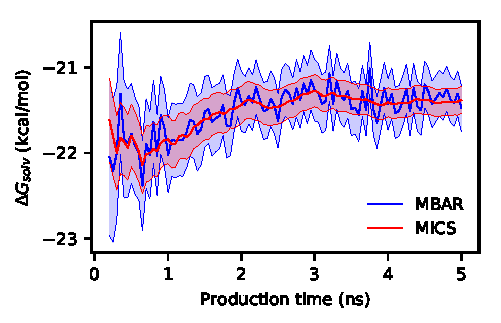
\includegraphics{glucose_sample_size.pdf}
	\caption{Free energies computed for sampled states as well as values perturbed for unsampled ones.}
\end{figure}

%\begin{figure}
%	\label{fig:overlap matrix}
%	\includegraphics{overlap_matrix.pdf}
%	\caption{Free energies computed for sampled states as well as values perturbed for unsampled ones.}
%\end{figure}

\begin{figure}
	\label{fig:glucose FEP}
	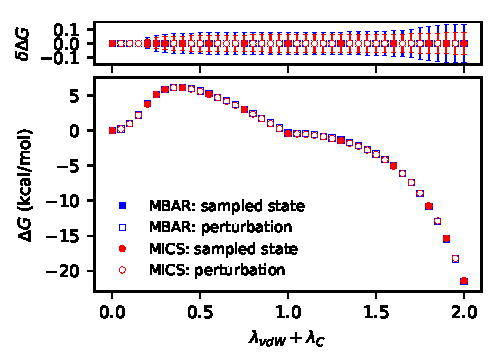
\includegraphics{glucose_fep.pdf}
	\caption{Free energies computed for sampled states as well as values perturbed for unsampled ones.}
\end{figure}


\begin{figure}
	\label{fig:composition analysis}
	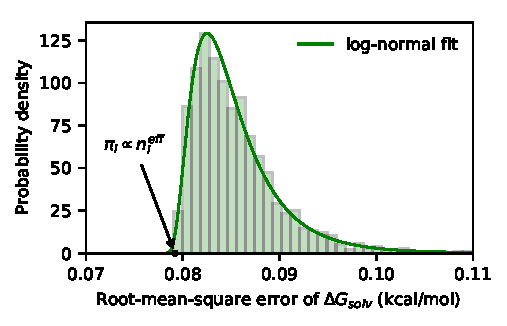
\includegraphics{composition_analysis.pdf}
	\caption{Free energies computed for sampled states as well as values perturbed for unsampled ones.}
\end{figure}


%From Ref.~\citenum{Shirts_2003_2}
%\begin{equation*}
%{\Delta G}_\text{solv} = RT \left[{\Delta f}_{a,b} - \ln \left(\frac{\avg{V}_b}{\avg{V}_a}\right)\right],
%\end{equation*}
%where subscripts $a$ and $b$ refer to the initial state (uncoupled solute) and to the final state (fully coupled solute), respectively. 
%
%\begin{figure}
%	\centering
%	\includegraphics{Figures/nelder_mead}
%	\caption{}
%	\label{fig:nelder_mead}
%\end{figure}


\subsection{Potential of Mean Force for a Host-Guest System}

WHAM method\cite{Ferrenberg_1989, *Kumar_1992} and implementation \cite{Grossfield_nodate}.

Cucurbit[7]uril. GAFF parameters \cite{Wang_2004}. AM1-BCC charges \cite{Jakalian_2000, *Jakalian_2002} using the Antechamber \cite{Wang_2006} as implemented in Ambertools 2017 \cite{Case_2017}.

%\begin{figure}
%	\label{fig:carboxylatopillar[5]arene}
%	\centering
%	\includegraphics[width=2.5in]{wp5_paraquat.png}
%	\caption{Host and guest molecule at their minimum-energy conformations according to the AM1 semi-empirical Hamiltonian. Left: a deca-carboxylatopillar[5]arene (wp5) anion. Right: a 1,1'-dimethyl-4,4'-bipyridinium (paraquat) cation.}
%\end{figure}

\begin{figure}
	\label{fig:carboxylatopillar[6]arene}
	\centering
	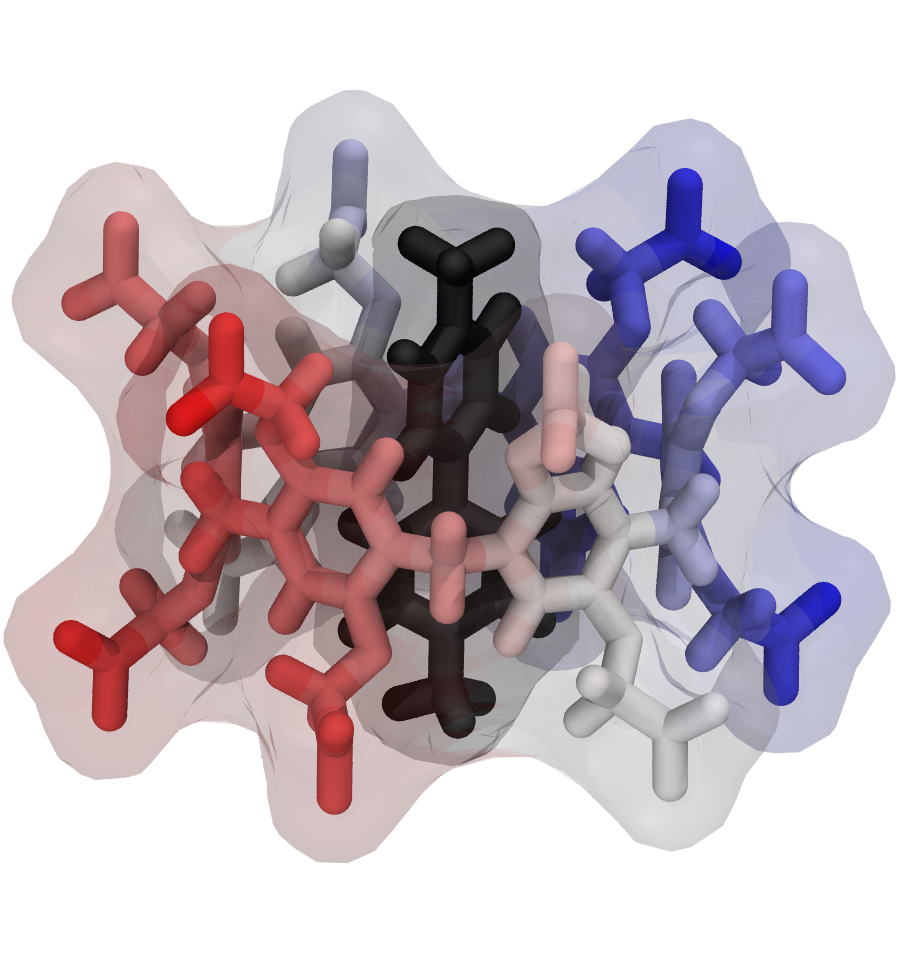
\includegraphics[width=2.5in]{wp6_paraquat.png}
	\caption{Host (dodeca-carboxylato-pillar[6]arene anion, in colors) and guest (1,1'-dimethyl-4,4'-bipyridinium cation, also known as paraquat, in dark gray) at their individual minimum-energy conformations according to the AM1 semi-empirical Hamiltonian.}
\end{figure}

\section{Conclusion}

Free-energy perturbation is an accurate method when the typical configurations of the target state form a significant subset of the typical configurations of the sampled state.

We tried to interpret different methods simply as distinct choices of a reduced potential $u_0(x)$ for the reference state, expressed as an analytical function $u_0 = u_0(u_1,\dots,u_n)$.

Possible development: reweighting and perturbation involving simultaneously two or more unsampled states, so that  

\begin{acknowledgement}

The author acknowledges the financial support of Petrobras (project code CENPES 16113).

\end{acknowledgement}

\bibliography{mics}

\end{document}